
%%%%%%%%% SUMMARY -- 1 page, third person
% e.g:  "The PI will prove" not "I will prove"

%Introduction / Summary (1 page).  The following information is typically included in proposal introductions for this 
%grant. The summary should lead to the proposal body but it should also be a self-contained document, 
%summarizing what is being proposed and why.   
 
% Provide appropriate background that sets the context for the problem and the objectives. 
%State the specific problem (may also be thought of as a need, central research question, or hypothesis) 
%your research will address. 
% State the objectives of the proposed research. 
%State any limits of the proposed research  (may not be needed). 
%Summarize the research methods you will use to achieve research objectives (if clearly covered elsewhere 
%in the introduction, a separate section may not be needed). 


%\required{Project Summary}
\section{Project Summary}
% This should be a brief statement of the problem you plan to address.
% It should look something like an abstract. 
In today's scientific environment, there is a growing focus on data storage and
processing. Some of the largest problems scientists face are related to the data
deluge, and the inability to conceptualize problems and solutions from large
tracts of data. The result is many attempts by scientific professionals to 
design software, leading to many bad software designs. Vast amounts of 
expensively collected data never get processed, 
because the software designs take so much maintenance. Data is often duplicated,
often in different locations, lost, or never makes it from collection to 
analysis. The overall lack of system designs to handle the data further 
hinders analysis.

This proposal is for a project that helps solve these design problems for 
many scientists. The project is a data harvester and organizer tool. It
is a local web interface that allows scientists to collect, query, organize, 
and share data with other researchers.
Many of these scientists work with similar data sets, ask different 
questions, and need immediate search tools. The proposed tool would first allow 
users to visualize and filter data, and secondly prepare and ship the data
off for analysis. It also helps users visualize data graphically, to 
help the conceptualize, organize, and refine data, before transporting and 
processing it. This 
project proposes using PTAG and othe ecological data sets from the Columbia 
Basin to test design, but should be exdendable to many different users with very
different data sets.

The tool will not overlap with the functionality of existing tools like 
PTAGIS or DART. It will carefully handle data sharing,
choosing opt-in, lock-down policies by default.

\subsection{Background}
%this section needs more stats and citations
In the Columbia Basin today, millions of federal dollars are spent on PTAG 
and othe systems to collect environmental data. 
This data includes fish location, ecological community composition, and 
abiotic data. Yet, the project 
results from most research are far from concrete. Despite the lack of 
understandable results, important decisions that affect the local environment 
and economy have to be made. Decisions like whether or not to conduct 
major habitat restoration projects. 

%We should cite something other study / examples in the basin. Foster's talk
% just sticks in my head as a good example
The Columbia Basin is just one small example. Bioinformatics is another 
data intesive study that generates more data that it can process. Its 
%is this 10%? It may be lower
estimated that less than 10\% of the data collected by bioinformatic 
researchers at the University of Idaho actually makes it through proccessing
\cite{foster}. The rest has to be filtered as best as can be managed, and the 
low value data trimmed out. The problem with 10\% data use, is that not just 
the fat, but the meat and bone has to be cut away. Either significantly more
data must be analyzed, or significantly less should be collected. At the very
least, storing the data in an easily readable format can show where the 
gaps are. So far, our experience and research shows similar shortfalls in 
data analysis in the Columbia Basin.

\subsection{Problem Statement}
One of the biggest problems researchers in the Columbia Basin have is getting
their data somewhere meaningful. Central databases like PTAGIS offer a 
central storage and clients can push data there, but they don't offer useful
tools for managing data. Once the data is pushed, it is hard to access and
manipulate. 
%stuff to massage
% I hate to get rid of the next bit, because it is some of the buzz that the
% project approvers are looking for. Can we work this verbage in without it
% being a priority / main focus?
Researchers are often in remote locations, and have low bandwidth
connections. 
% end stuff to massage
Creating a robust tool will guarantee ease of use for the data, no matter
the location.

Many researchers have significant data management tasks before even thinking 
about pushing data to the cloud. Once they are ready, they need seemless ways to
synchronize data to and from the cloud. They also may want to query their data,
and filter it into small subsets. Most researchers don't have time to learn
new programming language or interfaces. They need a data management tool 
that has a user 
interface that is familiar to use cases they already understand. Once they
have created a data subset, they will want to share it, save it, copy it, 
and compare it with other data sets. Getting the right data to the right place 
in the right amount of time is crucial.

\subsection{Objectives}

\begin{figure}[!h]
        \begin{center}
		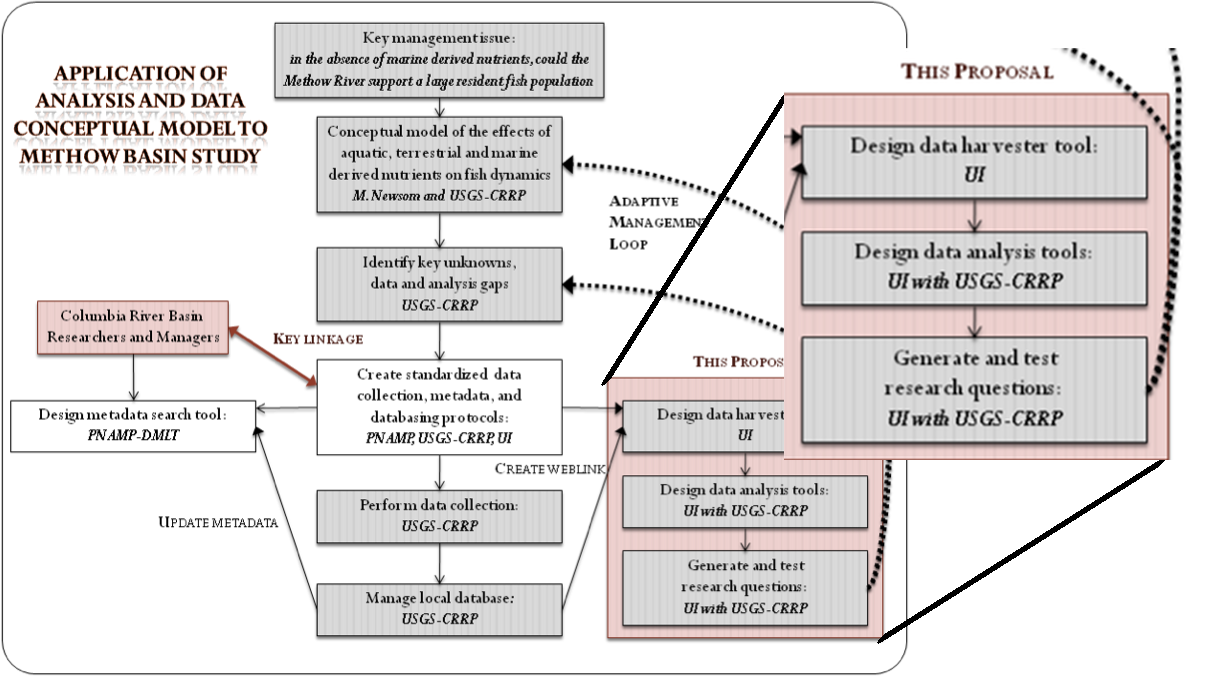
\includegraphics[width=120mm]{images/combo_proposal}
                \caption{This proposal software's application domain in DE-CRRP}
                \label{combo_proposal}
        \end{center}
\end{figure}

The proposed project will tackle the UI data harvester portion of the grant 
funded USGS-CRRP project (Figure \ref{combo_proposal}), directed by Alex 
Fremier of the UI College of Natural Resources. The data management tool
will be a web-like GUI that can be installed locally on the clients' computers.
The tool will contain a expandable meta data server 
that can be connected to others, for a \textbf{decentralized} data storage
cloud. The cloud will consist of the many instances of the tool, acting as a
cloud of 
\textbf{decentralized databases}. It will contain an interface to an existing 
or custom \textbf{networking protocol} that will allow for many different data 
formats to be synchronized across the cloud. The project will also have graphic
interfaces for \textbf{seamless data management}.

The decentralized cloud model allows some serious advantages to researchers.
They can see exactly what their data looks like, before they submit it.
They can filter out bad data before it consumes bandwidth, and can retract
undesirable data from the cloud, even after synchronizing it. It also frees
them from central storage service management and fees, and 
\textbf{encourages internode and inter-research communication}. 
The tool can be setup
on multiple hosts, and can be used for the benefits of 
the centralized cloud model. Each client can decide what topology suites them 
best.

The decentralized cloud model implements a distributed database model.
Distributed databases increase availability and reliability. They are more
easily expandable, and can better protect from data loss from local disasters or
malicious attacks. Moving data to where it is in highest demand also increases
query performance. Offloading archive data to remote site with more 
resources preserves local resources. Replicated datasets can guarantee 
better availability. By staging data locally and filtering it before allowing
it to be exchanged, the autonomy of the organization is better preserved. 

%probably some specific network protocols, like SOAP, etc, should be mentioned
%Alex, the network protocol doesn't have to apply just to low bandwidth users
%, but also to large data transfers
The network protocol will allow incremental synchronization of data from host
to host, even in less reliable environments. The tool will create
an \textbf{outreach} from researchers in high availability areas to those
in low availability, low bandwidth areas, and back. The network protocol
will have support for major data formats (i.e. SQL, CSV, more), and allow
users to send incremental pieces of the data. In the case of very large 
data sets or low bandwidth, the receiver of the data can still use it. Whether 
the data takes more time to transfer, or never completes.

The seamless interface will allow users to sort their data needing only 
basic knowledge of computers. Users will be able their mouse to select
datasets and apply filters to them. The tool will allow them to query local or
remote data, or to dynamically join both. Queries will create data subsets that
users can bring to a workspace. The tool will be able to sort data however
the user likes, on the fly. It will then be able to graph the ranges in 
the subset in most ways the user could want to sort them.

Once the user has manipulated their data subset to their satisfaction, they
will be able to save it in the meta data server's format, or in a set of major
data formats. The tool will also have analysis modules that will allow them
to run analysis on the local host. These modules will be extensible to running 
analysis jobs on other designated compute hosts, like workstations, clusters,
or even Amazon's EC2. The tool will come only with basic functionality for 
local analysis modules, but will be extensible to the heavier compute options.
%\required{Intellectual Merit}
% This is why your project is interesting and will help further
% knowledge in the field of mathematics. 

%\required{Broader Impacts}
% There are 4 kinds of broader impacts.
% 1. advance discovery and understanding while promoting teaching,
% training and learning
% 2. broaden the participation of underrepresented groups
% 3. disseminated broadly to enhance scientific and technological
% understanding
% 4. benefits of the proposed activity to society

